% This is samplepaper.tex, a sample chapter demonstrating the
% LLNCS macro package for Springer Computer Science proceedings;
% Version 2.20 of 2017/10/04
%
\documentclass[runningheads]{llncs}
%
\usepackage{graphicx}
% Used for displaying a sample figure. If possible, figure files should
% be included in EPS format.
%
% If you use the hyperref package, please uncomment the following line
% to display URLs in blue roman font according to Springer's eBook style:
% \renewcommand\UrlFont{\color{blue}\rmfamily}

\begin{document}
%
\title{Planification multicast pour optimiser la consommation 
d'\'energie avec des contraintes de d\'elais}
%
%\titlerunning{Abbreviated paper title}
% If the paper title is too long for the running head, you can set
% an abbreviated paper title here
%
\author{Isma\"il Bagayoko}
%
% \authorrunning{I. Bagayoko et al.}
% First names are abbreviated in the running head.
% If there are more than two authors, 'et al.' is used.
%
\institute{Universit\'e du Qu\'ebec \`a Montr\'eal \\
\email{bagayoko.ismail@courrier.uqam.ca}\\
\url{} }
%
\maketitle              % typeset the header of the contribution
%
\begin{abstract}
Ces dernières années, le trafic mobile a considérablement augmenté. 
Il y a une similitude dans les demandes de données au niveau station 
de base. Les requêtes pour les mêmes données sont à des intervalles 
de juste quelques microsecondes, la station de base se trouve à faire des 
opérations très répétitives. 

L'ancienne méthode où les requêtes sont servis une à la fois ne 
fonctionne plus, il n'est pas rentable en matière de ressources 
(ex: énergie). C'est là qu'intervient la multi-diffusion (multicast), 
elle consiste à servir plusieurs requêtes en un seul envoi (réponse).
Il faut attendre de recevoir  plusieurs requêtes pour les servir en 
un seul envoi. On s'aperçoit tout de suite que l'idéal c'est d'attendre 
infiniment et servir. Les premières requêtes vont beaucoup attendre pour 
être servis.

Il y a un compromis à  faire ici, plus on attend plus on économise en 
ressources mais plus l'on attend plus nous perdons en matière de qualité 
de service. Un exemple d'utilisation est un fournisseur d'accès internet 
qui veut minimiser l'utilisation des ressources mais respecter les délais 
payés par les clients.un

La multi-diffusion bien qu'existe depuis très longtemps, au cours des 
dernières années elle a suscité beaucoup d'intérêt dû aux nombreux 
avantages qu'elle apporte: le coût en énergie, l'utilisation efficace 
du canal et bien d'autres.

The abstract should briefly summarize the contents of the paper in
150--250 words.

\keywords{First keyword  \and Second keyword. }
\end{abstract}
%
%
%
\section{Introduction}
\section{Formulation du problème}
Nous considérons un ensemble $R$ de requêtes défini comme 
$R = \{(a, d, m, e )_i\} $ où :
\begin{itemize}
    \item $a_i$ est l'instant d'arriver de la requête $i$
    \item $d_i$ est le dernier instant que peut tolérer la requête $i$
    \item $m_i$ est l'identifiant du contenu (message) demandé par la requête  $i$
    \item $e_i$ l'énergie nécessaire pour répondre à la requête $i$
\end{itemize} 

On définit les variables de décision:
\begin{itemize}
    \item $x_i$ est l'instant d'envoi de la requête $i$ à  déterminer 
    \item $y_m$ est l'instant d'envoi du message  $m$ à  déterminer 
    \item $E_t$ représente l'énergie consommée a un instant $t$
    \item $E_t^m$ représente l'énergie consommée a un instant $t$ pour 
    le message $m$
\end{itemize}

Nous consid\'erons les deux cas suivant lorsqu'un seul contenu o\`u plusieurs 
sont disponibles pour la multidiffusion est disponible au niveau de la 
station de base.
\subsubsection{Un message}
\[
    \begin{array}{cc}
         \textbf{minimiser} &  \sum\limits_{t} E_t\\
         \textbf{Sous contraintes} & \\
         & E_t = \max\limits_{x_i=t} e_i \\
         & a_i \leq x_i \leq d_i\\
    \end{array}
\] 
\subsubsection{Plus d'n message}
\section{Solutions propos\'es }
\subsection{Une solution na\"ive }
\subsection{Une m\'ethode gloutonne}

\subsection{Un algorithme g\'en\'etique}


\subsubsection{Sample Heading (Third Level)} Only two levels of
headings should be numbered. Lower level headings remain unnumbered;
they are formatted as run-in headings.

\paragraph{Sample Heading (Fourth Level)}
The contribution should contain no more than four levels of
headings. Table~\ref{tab1} gives a summary of all heading levels.

\begin{table}
\caption{Table captions should be placed above the
tables.}\label{tab1}
\begin{tabular}{|l|l|l|}
\hline
Heading level &  Example & Font size and style\\
\hline
Title (centered) &  {\Large\bfseries Lecture Notes} & 14 point, bold\\
1st-level heading &  {\large\bfseries 1 Introduction} & 12 point, bold\\
2nd-level heading & {\bfseries 2.1 Printing Area} & 10 point, bold\\
3rd-level heading & {\bfseries Run-in Heading in Bold.} Text follows & 10 point, bold\\
4th-level heading & {\itshape Lowest Level Heading.} Text follows & 10 point, italic\\
\hline
\end{tabular}
\end{table}


\noindent Displayed equations are centered and set on a separate
line.
\begin{equation}
x + y = z
\end{equation}
Please try to avoid rasterized images for line-art diagrams and
schemas. Whenever possible, use vector graphics instead (see
Fig.~\ref{fig1}).

\begin{figure}
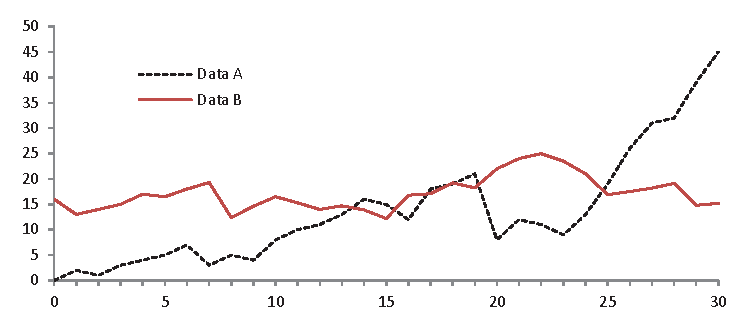
\includegraphics[width=\textwidth]{fig1.eps}
\caption{A figure caption is always placed below the illustration.
Please note that short captions are centered, while long ones are
justified by the macro package automatically.} \label{fig1}
\end{figure}

\begin{theorem}
This is a sample theorem. The run-in heading is set in bold, while
the following text appears in italics. Definitions, lemmas,
propositions, and corollaries are styled the same way.
\end{theorem}
%
% the environments 'definition', 'lemma', 'proposition', 'corollary',
% 'remark', and 'example' are defined in the LLNCS documentclass as well.
%
\begin{proof}
Proofs, examples, and remarks have the initial word in italics,
while the following text appears in normal font.
\end{proof}
For citations of references, we prefer the use of square brackets
and consecutive numbers. Citations using labels or the author/year
convention are also acceptable. The following bibliography provides
a sample reference list with entries for journal
articles~\cite{ref_article1}, an LNCS chapter~\cite{ref_lncs1}, a
book~\cite{ref_book1}, proceedings without editors~\cite{ref_proc1},
and a homepage~\cite{ref_url1}. Multiple citations are grouped
\cite{ref_article1,ref_lncs1,ref_book1},
\cite{ref_article1,ref_book1,ref_proc1,ref_url1}.
%
% ---- Bibliography ----
%
% BibTeX users should specify bibliography style 'splncs04'.
% References will then be sorted and formatted in the correct style.
%
% \bibliographystyle{splncs04}
% \bibliography{mybibliography}
%
\begin{thebibliography}{8}
\bibitem{ref_article1}
Author, F.: Article title. Journal \textbf{2}(5), 99--110 (2016)

\bibitem{ref_lncs1}
Author, F., Author, S.: Title of a proceedings paper. In: Editor,
F., Editor, S. (eds.) CONFERENCE 2016, LNCS, vol. 9999, pp. 1--13.
Springer, Heidelberg (2016). \doi{10.10007/1234567890}

\bibitem{ref_book1}
Author, F., Author, S., Author, T.: Book title. 2nd edn. Publisher,
Location (1999)

\bibitem{ref_proc1}
Author, A.-B.: Contribution title. In: 9th International Proceedings
on Proceedings, pp. 1--2. Publisher, Location (2010)

\bibitem{ref_url1}
LNCS Homepage, \url{http://www.springer.com/lncs}. Last accessed 4
Oct 2017
\end{thebibliography}
\end{document}
